%Hojear con intención: qué es Wigner-Dyson vs Poisson, Berry-Tabor, semiclásico. No demostrar, solo intuición y ejemplos gráficos del review.
%1 mini-figura prestada del review (redibujada) y 5 líneas que relacionen RMT con ETH.

\begin{frame}

\frametitle{Non-chaotic vs chaotic system}
    
    \begin{block}{}
    Example of trajectorie of particle bouncing in non-chaotic and chaotic system. the system b) is called Bunimovich stadium
    \end{block}

\begin{figure}
    \centering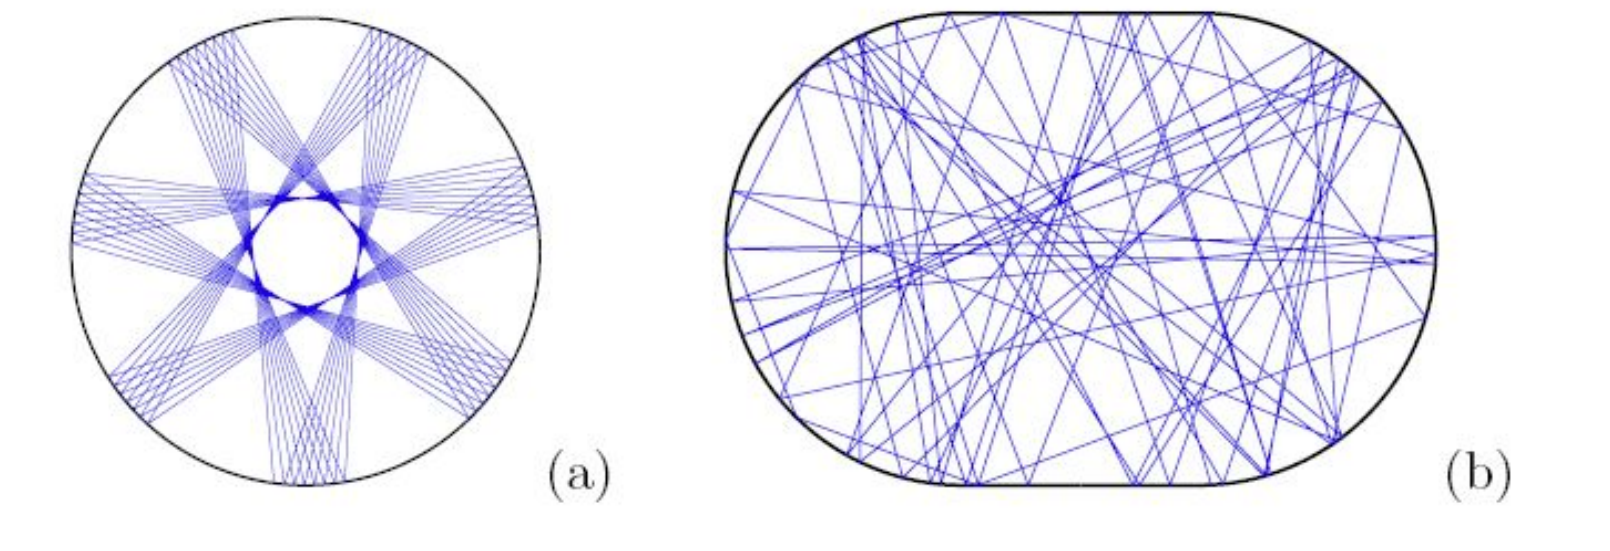
\includegraphics[width=\textwidth]{chaos.png}
\end{figure}

\end{frame}

% --- Slide 1: Wigner–Dyson vs Poisson ---
\begin{frame}[plain]
    \frametitle{Level Statistics: Wigner–Dyson vs. Poisson}
    
    \begin{block}{}
    Chaotic systems show \textbf{level repulsion} (Wigner–Dyson),  
    while integrable ones display \textbf{uncorrelated levels} (Poisson).  
    This contrast is the main signature of quantum chaos.
    \end{block}
    
    \begin{figure}
        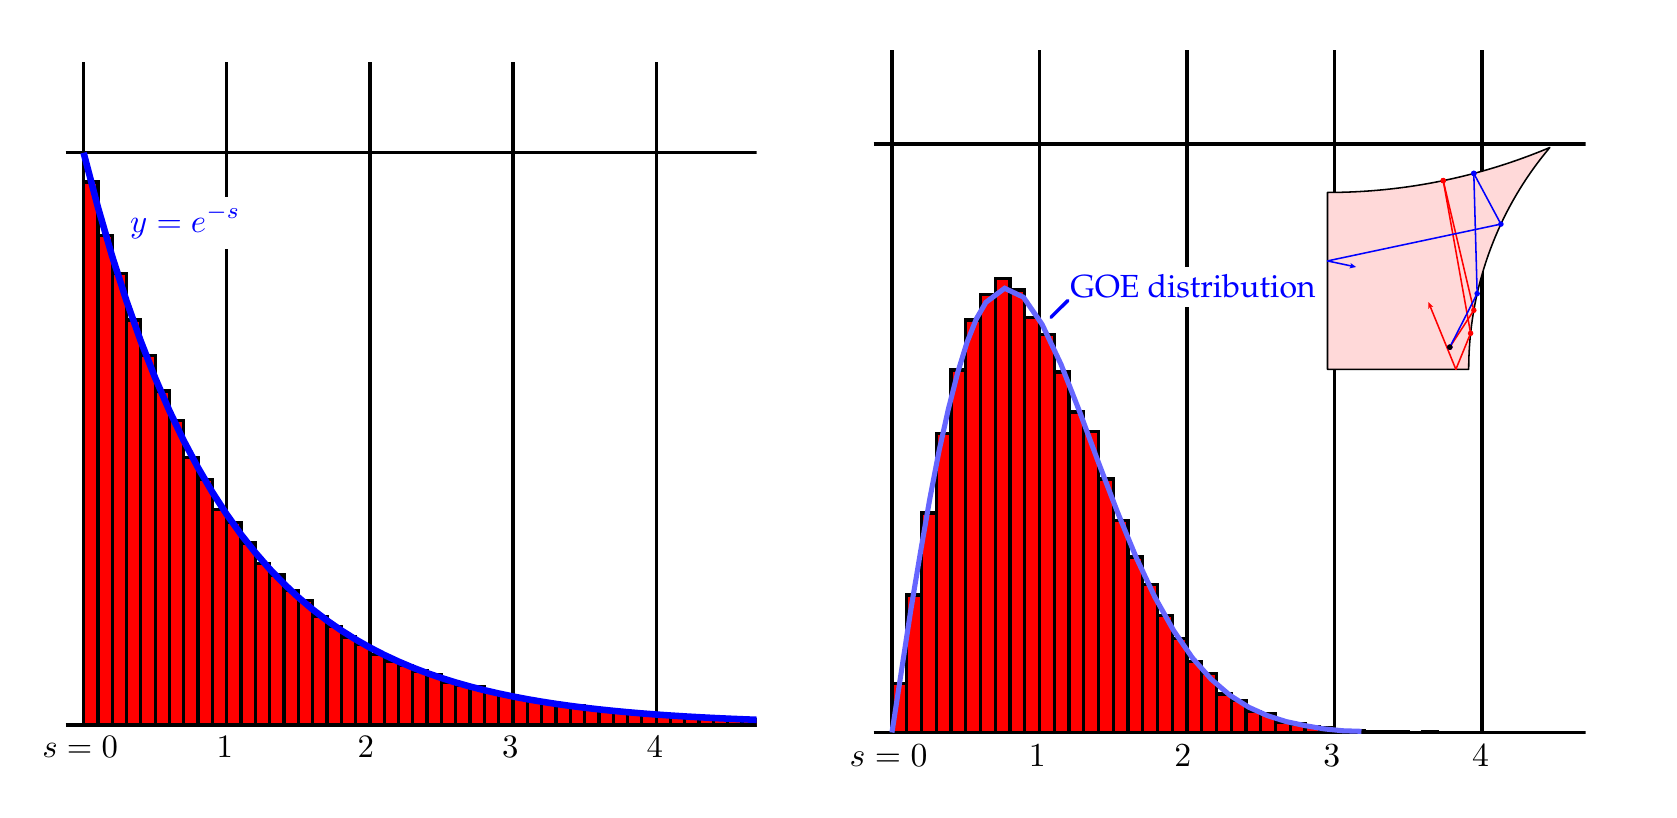
\includegraphics[width=\textwidth, keepaspectratio]{distribution.png}
    \end{figure}
\end{frame}

\begin{frame}

  \frametitle{Equations: Poisson vs WD-GOE}
  
  \begin{block}{Poisson Distribution (Integrable Systems)}
  Describes uncorrelated energy levels. There is no level repulsion, meaning levels can be arbitrarily close.
  \[
  P_0(\omega) = e^{-\omega}
  \]
  \end{block}
  
  \begin{block}{Wigner-Dyson GOE (Chaotic Systems - Wigner Surmise)}
  Describes chaotic systems with time-reversal symmetry. The linear term $\omega$ shows level repulsion.
  \[
  P_1(\omega) = \frac{\pi}{2}\omega e^{-\frac{\pi}{4}\omega^2}
  \]
  \end{block}

\end{frame}

% --- Slide 2: Berry–Tabor ---
\begin{frame}[plain]
    \frametitle{Semiclassics I: Berry–Tabor Conjecture}
    
    \begin{block}{}
    Quantum systems with a \textbf{classically integrable} counterpart  
    (e.g., a particle in a rectangular box) exhibit \textbf{Poisson statistics}.
    \end{block}

    \begin{figure}
        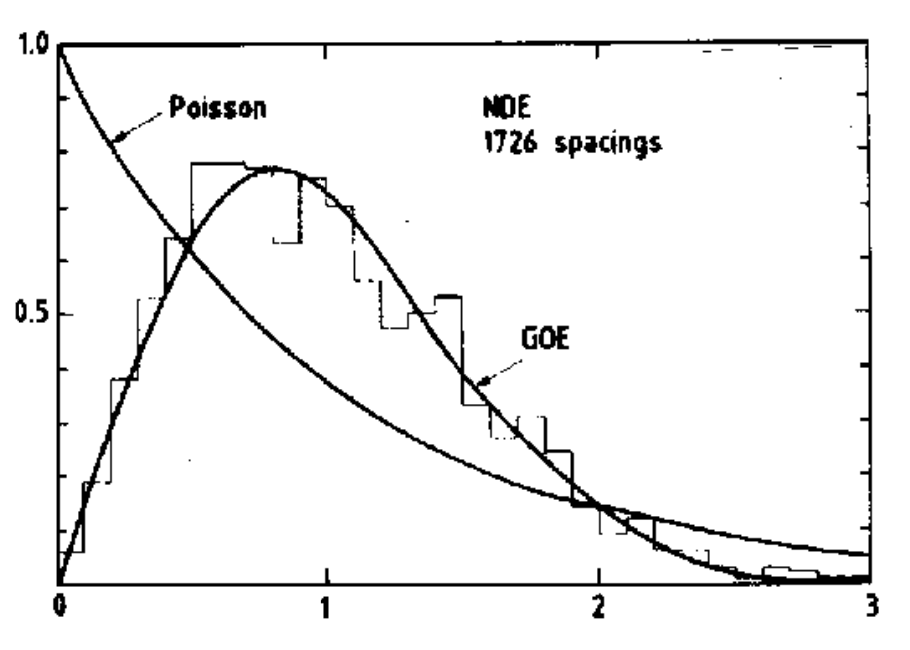
\includegraphics[width=0.8\textwidth, keepaspectratio]{Wigner-Dyson-Poisson Statistics.png}
    \end{figure}
\end{frame}

% --- Slide 3: BGS Conjecture ---
\begin{frame}[plain]
    \frametitle{Semiclassics II: BGS Conjecture}
    
    \begin{block}{}
    Quantum systems with a \textbf{classically chaotic} counterpart  
    follow \textbf{Random Matrix Theory (RMT)} level statistics.
    \end{block}

    \begin{figure}
        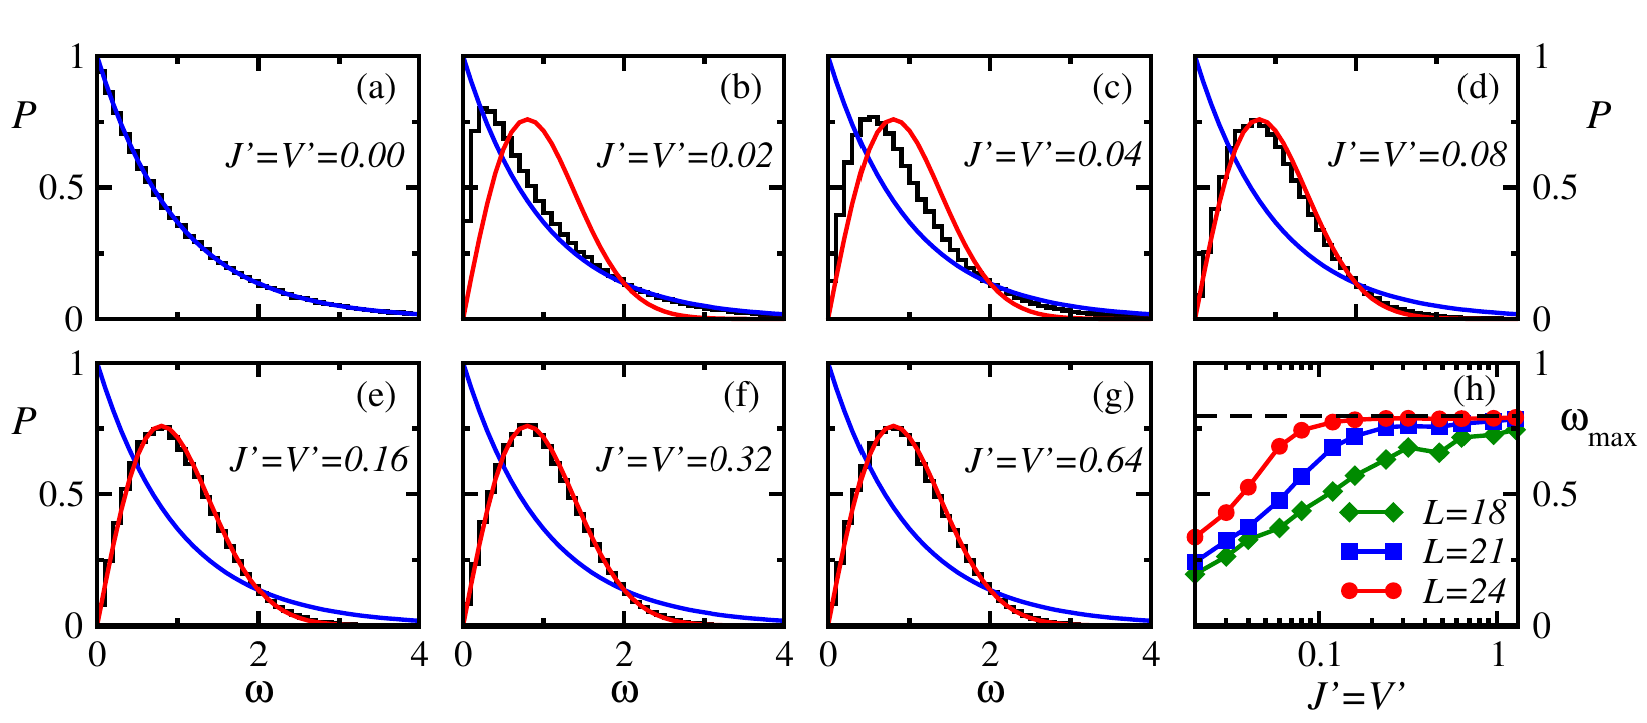
\includegraphics[width=\textwidth, keepaspectratio]{spacing.png}
    \end{figure}
\end{frame}

% --- Slide 4: From RMT to ETH ---
\begin{frame}
    \frametitle{From Random Matrices to Thermalization}
    
    \begin{columns}[T,onlytextwidth]
        \begin{column}{0.48\textwidth}
            \begin{block}{Random Matrix Theory (RMT)}
                \begin{itemize}
                    \item Wigner–Dyson statistics  
                    \item Random eigenvectors  
                    \item $O_{mn} \approx \bar{O}\delta_{mn} + \text{noise}$
                \end{itemize}
            \end{block}
        \end{column}

        \begin{column}{0.48\textwidth}
            \begin{block}{Eigenstate Thermalization Hypothesis (ETH)}
                \begin{itemize}
                    \item Also Wigner–Dyson  
                    \item Eigenstates are “thermal”  
                    \item $O_{mn} = O(\bar{E})\delta_{mn} + e^{-S/2}f(\bar{E},\omega)R_{mn}$
                \end{itemize}
            \end{block}
        \end{column}
    \end{columns}
    
    \vspace{0.4cm}
    \begin{alertblock}{Key Idea}
    ETH extends RMT by adding physical structure:  
    observable matrix elements become smooth functions of energy,  
    providing a microscopic explanation for thermalization  
    in isolated many-body systems.
    \end{alertblock}
\end{frame}
